% =============================================================================
% 17-803 Empirical Methods Guest Lecture
% An Introduction to Causal Inference on Observational Data
% Hao He, Carnegie Mellon University
% =============================================================================
\documentclass[aspectratio=169, 12pt]{beamer}

% --- Packages ----------------------------------------------------------------
\usepackage{amsmath,amssymb}
\usepackage{graphicx}
\usepackage{tikz}
\usetikzlibrary{arrows.meta, positioning, shapes.geometric, calc, decorations.pathreplacing}
\usepackage{booktabs}
\usepackage{hyperref}
\usepackage{xcolor}

% --- Colors ------------------------------------------------------------------
\definecolor{creambar}{HTML}{FFF2CC}
\definecolor{goldfoot}{HTML}{F5C34B}
\definecolor{emphred}{HTML}{CC0000}
\definecolor{footgray}{HTML}{999999}
\definecolor{linkblue}{HTML}{0563C1}
\definecolor{lightgray}{HTML}{D9D9D9}
\definecolor{boxgray}{HTML}{BFBFBF}

% --- Beamer configuration ----------------------------------------------------
\setbeamertemplate{navigation symbols}{}
\setbeamerfont{frametitle}{size=\Large, series=\mdseries}
\setbeamercolor{frametitle}{fg=black}
\setbeamertemplate{itemize item}{\textbullet}
\setbeamertemplate{itemize subitem}{\textbullet}
\setbeamertemplate{itemize subsubitem}{\textbullet}
\setbeamersize{text margin left=0.5cm, text margin right=0.5cm}
\setbeamertemplate{frametitle}{%
  \vskip0.3cm%
  \noindent\insertframetitle%
}
\setlength{\leftmargini}{1.2em}
\setlength{\leftmarginii}{1.2em}

% --- Convenience macros ------------------------------------------------------
\newcommand{\redt}[1]{\textcolor{emphred}{#1}}
\newcommand{\bluet}[1]{\textcolor{linkblue}{#1}}

% Placeholder for images: gray box with caption
\newcommand{\placeholderimg}[3]{%
  % #1 = width, #2 = height, #3 = caption
  \begin{tikzpicture}
    \draw[thick, dashed, gray] (0,0) rectangle (#1,#2);
    \node[text=gray, font=\small, align=center] at (#1/2,#2/2) {#3};
  \end{tikzpicture}%
}

% --- Footer with gold gradient -----------------------------------------------
\newcommand{\footertext}{An Introduction to Causal Inference on Observational Data}

\setbeamertemplate{footline}{%
  \begin{tikzpicture}[remember picture,overlay]
    \fill[creambar]
      (current page.south west) rectangle ([yshift=0.55cm]current page.south east);
    \node[anchor=south west, inner sep=0pt, text=footgray, font=\fontsize{7.5}{9}\selectfont]
      at ([xshift=0.4cm, yshift=0.15cm]current page.south west)
      {\footertext};
    \node[anchor=south east, inner sep=0pt, text=black, font=\fontsize{8}{10}\selectfont]
      at ([xshift=-0.4cm, yshift=0.15cm]current page.south east)
      {\insertframenumber};
  \end{tikzpicture}%
}

% --- Title page (custom) -----------------------------------------------------
\defbeamertemplate*{title page}{custom}[1][]{%
  
\begin{tikzpicture}[remember picture,overlay]
    % Cream sidebar on the left
    \fill[creambar] (current page.north west) rectangle ([xshift=2.5cm]current page.south west);
  \end{tikzpicture}%
  \vspace{0.6cm}
  \hspace{2.4cm}%
  \begin{minipage}{0.73\textwidth}
    {\small 17-803 Empirical Methods Guest Lecture}\\[1.2cm]
    {\fontsize{22}{22}\selectfont An Introduction to Causal Inference}\\[0.3cm]
    {\fontsize{22}{22}\selectfont on Observational Data}\\[0.1cm]
    \rule{0.55\textwidth}{0.5pt}\\[0.3cm]
    {\normalsize\textbf{Hao He}}\\[0.1cm]
    {\normalsize\textcolor{linkblue}{\href{mailto:haohe@andrew.cmu.edu}{haohe@andrew.cmu.edu}}}\\[0.1cm]
    {\normalsize Ph.D.\ Student in Software Engineering}\\[0.1cm]
    {\normalsize Carnegie Mellon University}
  \end{minipage}
}

% =============================================================================
\begin{document}
% =============================================================================

% ---------- Title Slide (no number) ------------------------------------------
{
\setbeamertemplate{footline}{}
\begin{frame}[plain]
  \titlepage
\end{frame}
}

% ---------- Slide 2 ----------------------------------------------------------
\begin{frame}{What you have learned from this class so far}
\begin{itemize}\setlength\itemsep{0.4em}
  \item Research Questions \& Theory Proposition
  \item Qualitative Methods
    \begin{itemize}
      \item Interviews
      \item Surveys
      \item Qualitative Data Analysis (open-coding, thematic analysis)
    \end{itemize}
  \item Quantitative Methods
    \begin{itemize}
      \item Controlled Experiments (comparing treatment \& control)
      \item Regression Modeling (correlations between X and Y holding Z constant)
    \end{itemize}
  \item Research Iteration and How to Handle with Controversies
  \item Anything you feel like maybe missing / unconvincing?
\end{itemize}
\end{frame}

% ---------- Slide 3 ----------------------------------------------------------
\begin{frame}{The intervention-outcome problem}
\begin{itemize}\setlength\itemsep{1.2em}
  \item Will attending CMU lead to higher incomes \redt{for you} in the future?
  \item What is the \redt{marginal disadvantage of you being women} in the tech industry?
  \item Will using Rust or Haskell \redt{help you write less bugs} in a real software project?
  \item Will using Claude Code \redt{help you or your project} write better code or worse code?
  \item \textbf{Why are these questions hard to answer?}
\end{itemize}
\end{frame}

% ---------- Slide 4 ----------------------------------------------------------
\begin{frame}{Why are intervention-outcome questions hard to answer?}
\begin{itemize}\setlength\itemsep{0.3em}
  \item Will attending CMU lead to higher incomes \redt{for you} in the future?
    \begin{itemize}
      \item Need two ``you''s, \textbf{the only difference} is one attending CMU and one not
    \end{itemize}
    \vspace{1em}
  \item What is the \redt{marginal disadvantage of you being women} in the tech industry?
    \begin{itemize}
      \item Need two ``you''s, \textbf{the only difference} is one being women and one being not
    \end{itemize}
    \vspace{1em}
  \item Will using Rust or Haskell \redt{help you write less bugs} in a real software project?
    \begin{itemize}
      \item Need two ``you''s working on two projects, \textbf{the only difference} is one written in Rust and the other written in (maybe) C++
    \end{itemize}
    \vspace{1em}
  \item Will using Claude Code \redt{help you or your project} write better code or worse code?
    \begin{itemize}
      \item Need two ``you''s working on two projects, \textbf{the only difference} is one uses Claude Code and the other does not use Claude Code
    \end{itemize}
    \vspace{1em}
\end{itemize}
\end{frame}

% ---------- Slide 5 ----------------------------------------------------------
\begin{frame}{The fundamental problem: \redt{No counterfactuals!}}
\begin{itemize}\setlength\itemsep{0.3em}
  \item Mathematically speaking:
    \begin{itemize}\setlength\itemsep{0.2em}
      \item Let $Y_i(1)$ be the outcome on $i$ when $i$ gets the intervention
      \item Let $Y_i(0)$ be the outcome on $i$ when $i$ does not get the intervention
      \item The true causal effect of \redt{intervening on $i$} is $Y_i(1) - Y_i(0)$
      \item However, for each $i$, \textbf{you either see $Y_i(1)$ or $Y_i(0)$, but never both!}
    \end{itemize}
  \item The workaround (attributing to the experiment pioneers in 1930s)
    \begin{itemize}\setlength\itemsep{0.2em}
      \item We \textbf{estimate} population level quantities like the average treatment effect (ATE)
      \[
        ATE = E[Y_i(1) - Y_i(0) \mid i \in P] = E[Y_i(1) \mid i \in P] - E[Y_i(0) \mid i \notin P]
      \]
      \item $P$ is the population of interest defined by the researcher (e.g., all human)
    \end{itemize}
\end{itemize}
\end{frame}

% ---------- Slide 6 ----------------------------------------------------------
\begin{frame}{Can you estimate counterfactuals through na\"ive comparisons?}
\begin{itemize}
  \item \textbf{Example Question} (note the change into population framing):
    \begin{itemize}
      \item Will attending CMU lead to higher incomes \redt{for an average person} in the future compared to \redt{not attending universities at all}?
    \end{itemize}
\end{itemize}

\begin{columns}[T]
  \column{0.45\textwidth}
  \centering
  % CMU salary histogram screenshot
  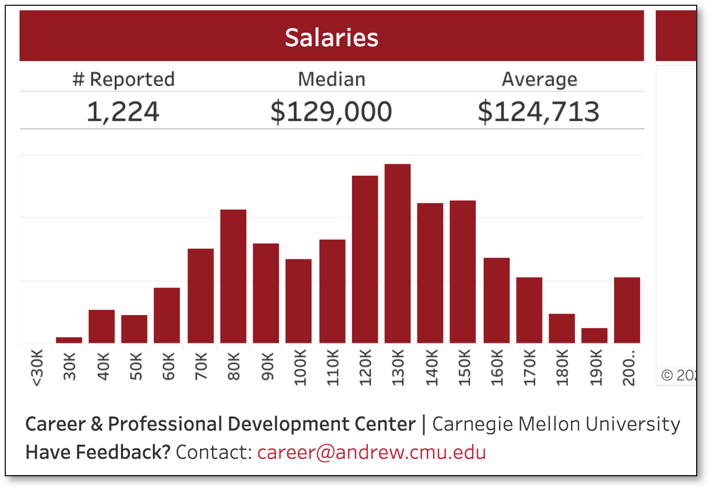
\includegraphics[height=4.2cm]{figures/cmu-salary.png}

  \column{0.55\textwidth}
  \centering
  % Google search result screenshot
  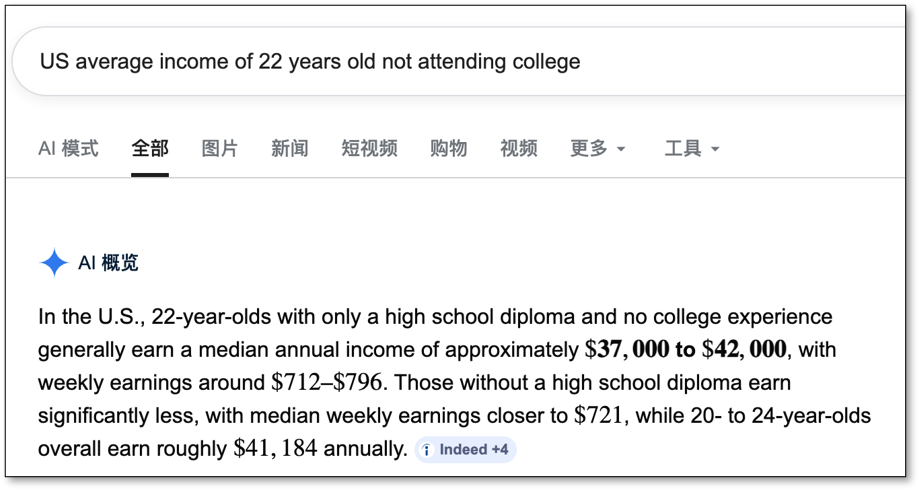
\includegraphics[height=4.2cm]{figures/google-income.png}
\end{columns}

\vspace{0.3cm}
\centering
People can expect to \redt{earn 3x income} if they can get into CMU! \textbf{Really}?
\end{frame}

% ---------- Slide 7 ----------------------------------------------------------
\begin{frame}{Decomposing \textbf{selection bias} --- And how to get rid of it?}

\vspace{-0.2em}
\begin{itemize}\setlength\itemsep{0.25em}
  \item \textbf{Selection bias}: CMU students would earn more \redt{even without CMU}
    \begin{itemize}
      \item Higher motivation, wealth, academic ability $\Rightarrow$ na\"ive 3$\times$ gap is inflated
    \end{itemize}
  \item \textbf{Mathematical decomposition}: Let $D_i\in\{0,1\}$ be whether unit $i$ is treated (e.g.\ attends CMU).
  The \textbf{na\"ive comparison} we are tempted to make:
  \[
    \underbrace{E[Y_i\mid D_i{=}1] - E[Y_i\mid D_i{=}0]}_{\text{na\"ive estimator}}
    \;=\; E[Y_i(1)\mid D_i{=}1] \;-\; E[Y_i(0)\mid D_i{=}0]
  \]

  \vspace{-0.2em}
  \noindent Add and subtract $E[Y_i(0)\mid D_i{=}1]$ (the \emph{unobserved} baseline of treated units):
  \[
    =\;\underbrace{E[Y_i(1)-Y_i(0)\mid D_i{=}1]}_{\text{ATT (true causal effect)}}
    \;+\;
    \underbrace{E[Y_i(0)\mid D_i{=}1] - E[Y_i(0)\mid D_i{=}0]}_{\redt{\text{selection bias}}}
  \]
  \item \textbf{To eliminate selection bias}: We need $E[Y_i(0)\mid D_i{=}1] = E[Y_i(0)\mid D_i{=}0]$
\end{itemize}

\end{frame}

% ---------- Slide 8 ----------------------------------------------------------
\begin{frame}{\redt{Randomization} + \redt{big numbers} eliminates selection bias}

\textbf{Randomization}: Assign treatment $D_i$ by a coin flip, \emph{independently} of everything in $i$:
\[
  D_i \;\perp\!\!\!\perp\; \bigl(Y_i(0),\, Y_i(1)\bigr)
\]

\vspace{-0.5em}
\noindent This independence kills selection bias immediately:
\[
  E[Y_i(0)\mid D_i{=}1] \;=\; E[Y_i(0)\mid D_i{=}0] \;=\; E[Y_i(0)]
\]

\vspace{-0.5em}
\noindent So the na\"ive estimator \emph{becomes} the ATE:
\[
  \underbrace{E[Y_i\mid D_i{=}1] - E[Y_i\mid D_i{=}0]}_{\text{na\"ive estimator}}
  \;=\; \underbrace{E[Y_i(1)-Y_i(0)]}_{\text{ATE}} \;+\; \underbrace{0}_{\text{bias} = 0}
\]

\vspace{-0.5em}
\begin{itemize}\setlength\itemsep{0.25em}
  \item \textbf{Big numbers}: sample averages $\hat{E}[\cdot] \xrightarrow{n\to\infty} E[\cdot]$ by the law of large numbers
  \item With enough units, $\bar{Y}_{\text{treated}} - \bar{Y}_{\text{control}}$ reliably estimates ATE (Fisher, Neyman, 1930s)
\end{itemize}

\end{frame}

% ---------- Slide 9 ----------------------------------------------------------
\begin{frame}{Well, can you really run a randomized controlled experiment on attending vs.\ not attending CMU?}

% Experiment flow diagram
\centering
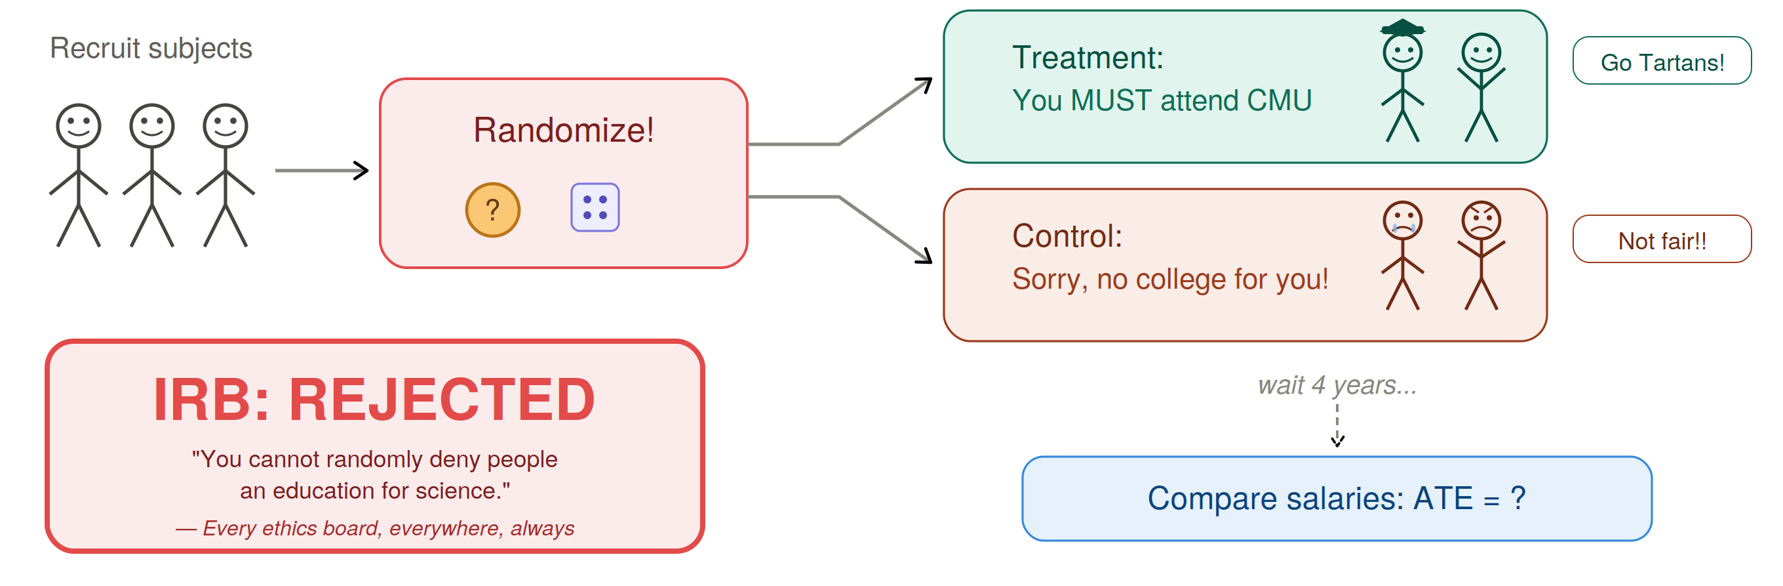
\includegraphics[width=\linewidth]{figures/experiment-cmu.png}

\begin{itemize}
  \item For a broad range of questions, experiments are just \redt{infeasible/unethical/too expensive}; this motivates an entire field of causal inference on \textbf{observational data}!
\end{itemize}
\end{frame}

% ---------- Slide 10 ---------------------------------------------------------
\begin{frame}{What about regressions we have learned in this class?}

% ---- Upper half: raw data table ----
\begin{center}
{\fontsize{10}{10}\selectfont
\begin{tabular}{crrrcrr}
  \toprule
  $i$ & GPA & SAT & Parent inc.\ (\$k) & CMU ($D_i$) & Income $Y_i$ (\$k) \\
  \midrule
   1 & 3.9 & 1520 & 180 & 1 & 119 \\
   2 & 3.7 & 1480 &  95 & 1 & 116 \\
   \vdots & \vdots & \vdots & \vdots & \vdots & \vdots \\
   998 & 2.9 & 1180 &  55 & 0 &  62 \\
   999 & 2.7 & 1150 &  48 & 0 &  57 \\
  1000 & 3.1 & 1290 &  72 & 0 &  73 \\
  \bottomrule
\end{tabular}
}
\end{center}

\vspace{0.2em}
\noindent\rule{\textwidth}{0.3pt}
\vspace{-0.5em}

% ---- Lower half: regression specification ----
\begin{itemize}
  \item \textbf{OLS regression} controlling for all observed confounders:
  \vspace{-0.5em}
  \[
    Y_i \;=\; \alpha + \beta\, D_i + \gamma_1\,\mathrm{GPA}_i + \gamma_2\,\mathrm{SAT}_i + \gamma_3\,\mathrm{ParentInc}_i + \varepsilon_i
  \]\vspace{-2em}
  \item Without controls: $\hat\beta \approx \$80$k \redt{(selection bias!)}, With controls: $\hat\beta \approx \$20$k
\end{itemize}
\end{frame}

% ---------- Slide 11 ---------------------------------------------------------
\begin{frame}{The \textbf{conditional ignorability} assumption (CIA)}

\textbf{CIA} (a.k.a.\ \emph{unconfoundedness}, \emph{selection on observables}):
\[
  \bigl\{Y_i(0),\,Y_i(1)\bigr\} \;\perp\!\!\!\perp\; D_i \;\Big|\; X_i
\]
\textit{Conditional on observed covariates $X_i$, treatment assignment is as good as random.}

\vspace{0.3em}
\textbf{Key consequence} (MHE Ch.\ 3, \S3.3): when CIA + \emph{common support} ($0 < P(D_i{=}1\mid X_i) < 1$) hold,
\[
  \underbrace{E\bigl[Y_i(1) - Y_i(0)\bigr]}_{\text{ATE}}
  \;=\;
  E\!\Bigl[\underbrace{E[Y_i \mid D_i{=}1,\, X_i] - E[Y_i \mid D_i{=}0,\, X_i]}_{\text{within-group comparison at each }X_i}\Bigr]
\]

\begin{itemize}\setlength\itemsep{0.25em}
  \item \textbf{Intuition}: at every value $X_i = x$, CIA makes $D_i$ random $\Rightarrow$ within-cell comparison is unbiased $\Rightarrow$ average over $x$ gives ATE
  \item \redt{CIA is the key identifying assumption} behind OLS, matching, IPW, and most observational estimators
  \item \textbf{Reference}: Angrist \& Pischke, \textit{Mostly Harmless Econometrics} (2009), Ch.\ 3 (esp.\ \S3.2--3.3)
\end{itemize}

\end{frame}

% ---------- Slide 12 ---------------------------------------------------------
\begin{frame}{How to justify the conditional ignorability assumption?}
\vfill
\centering
{\large\color{gray} [Board work]}
\vfill
\end{frame}

% ---------- Slide 13 ---------------------------------------------------------
\begin{frame}{Directed acyclic graphs (DAGs), confounders, colliders, and mediators}
\vfill
\centering
{\large\color{gray} [Board work: DAG structures]}
\vfill
\end{frame}

% ---------- Slide 14 ---------------------------------------------------------
\begin{frame}{Practical considerations and limitations of DAGs}
\vfill
\centering
{\large\color{gray} [Board work]}
\vfill
\end{frame}

% ---------- Slide 15 ---------------------------------------------------------
\begin{frame}{\textbf{Alternative A:} Design-based identification}
\vfill
\centering
{\large\color{gray} [Board work]}
\vfill
\end{frame}

% ---------- Slide 16 ---------------------------------------------------------
% This slide had no title visible, just the footer
\begin{frame}{}
\vfill
\centering
{\large\color{gray} [Board work / continuation]}
\vfill
\end{frame}

% ---------- Slide 17 ---------------------------------------------------------
\begin{frame}{\textbf{Alternative B:} Machine-learning-powered causal discovery}
\vfill
\centering
{\large\color{gray} [Board work]}
\vfill
\end{frame}

% ---------- Slide 18 ---------------------------------------------------------
\begin{frame}{\textbf{Summary:} The Modern Causal Inference Weaponry}
\vfill
\centering
{\large\color{gray} [Board work: summary of methods]}
\vfill
\end{frame}

% ---------- Slide 19 ---------------------------------------------------------
\begin{frame}{Example A: RDD on College Education}
\vfill
\centering
{\large\color{gray} [Board work / discussion]}
\vfill
\end{frame}

% ---------- Slide 20 ---------------------------------------------------------
\begin{frame}{Example B: The Impact of Gender in Tech}
\vfill
\centering
{\large\color{gray} [Board work / discussion]}
\vfill
\end{frame}

% ---------- Slide 21 ---------------------------------------------------------
\begin{frame}{Example C: The impact of using Rust/Haskell}
\vfill
\centering
{\large\color{gray} [Board work / discussion]}
\vfill
\end{frame}

% ---------- Slide 22 ---------------------------------------------------------
\begin{frame}{Example D: DiD on AI Coding Tool Adoption}
\vfill
\centering
{\large\color{gray} [Board work / discussion]}
\vfill
\end{frame}

% ---------- Slide 23 ----------------------------------------------------------
\begin{frame}{Recap}
\begin{enumerate}\setlength\itemsep{0.4em}
  \item Motivation: The intervention-outcome problem
  \item The fundamental problem of causal inference: No counterfactuals
  \item Selection bias \& why randomization helps (but isn't always feasible)
  \item Causal identification from observational data
    \begin{itemize}
      \item Regressions and conditional ignorability
      \item DAGs: confounders, colliders, and mediators
    \end{itemize}
  \item Alternative identification strategies
    \begin{itemize}
      \item Design-based identification
      \item ML-powered causal discovery
    \end{itemize}
  \item Summary of the causal inference toolbox
  \item Worked examples: RDD, gender in tech, Rust/Haskell, DiD on AI coding tools
\end{enumerate}
\end{frame}

% ---------- Slide 24 ----------------------------------------------------------
\begin{frame}{Further Readings and Recommendations}
\begin{columns}[T]
  \column{0.3\textwidth}
  \centering
  % Grid of book covers and logos
  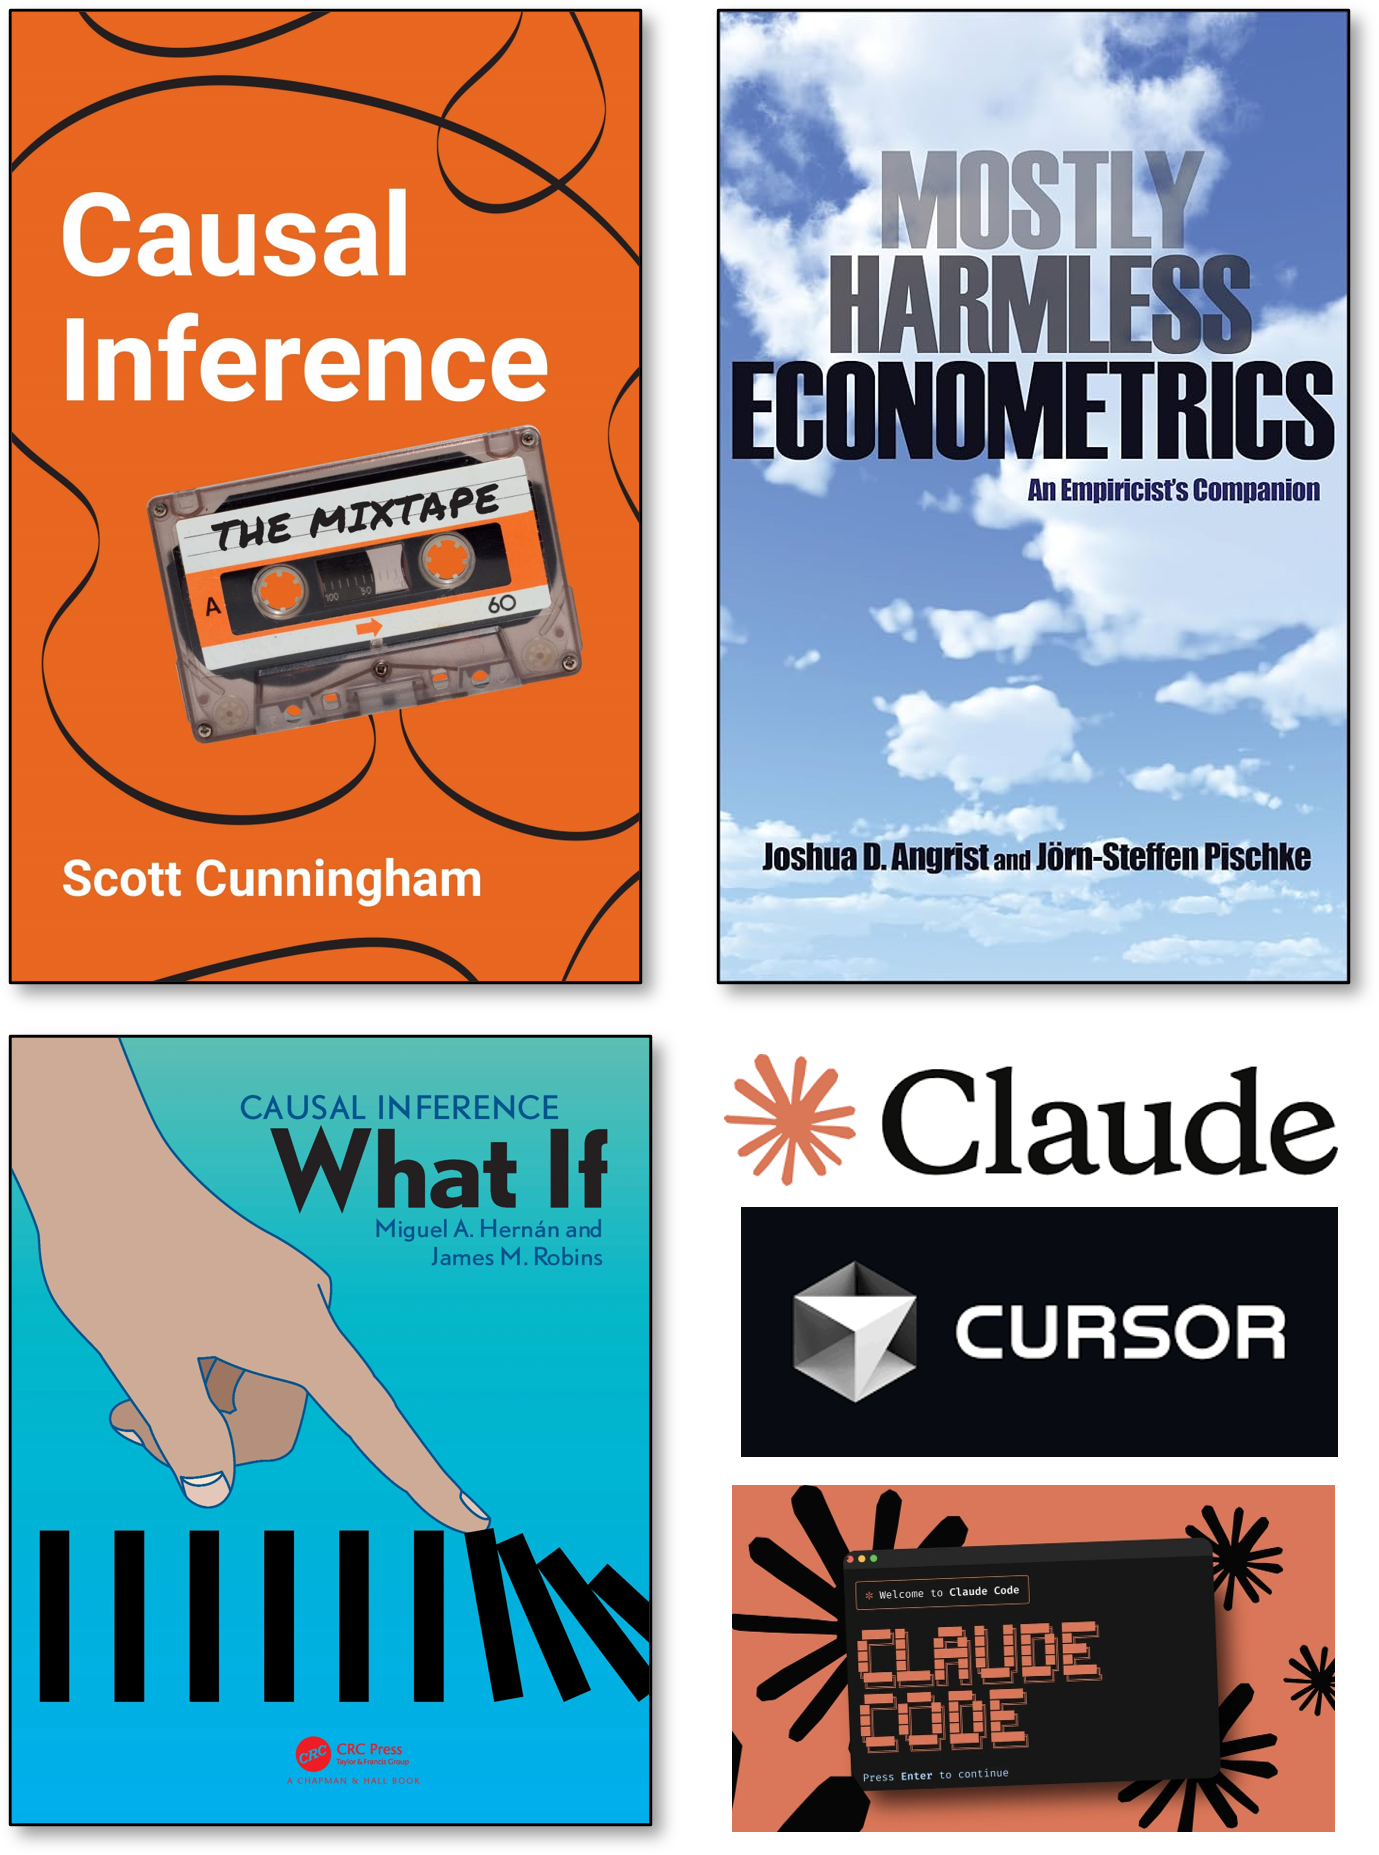
\includegraphics[width=\linewidth]{figures/book-covers.png}

  \column{0.65\textwidth}
  \begin{itemize}\setlength\itemsep{0.3em}
    \item \textbf{Mostly Harmless Econometrics: An Empiricist's Companion}, Angrist and Pischke
      \begin{itemize}
        \item Covering regressions for causal inference
      \end{itemize}
    \item \textbf{Causal Inference: The Mixed Tape}, Scott Cunningham, \textcolor{linkblue}{\url{https://mixtape.scunning.com/}}
      \begin{itemize}
        \item Covering design-based identifications
      \end{itemize}
    \item \textbf{Causal Inference: What If}, Hern\'an and Robins
      \begin{itemize}
        \item Covering DAGs and temporal structure methods
      \end{itemize}
    \item \textbf{Claude Opus 4.6 and its friends}
      \begin{itemize}
        \item Tremendously good teacher and coworker
        \item Great for brainstorming, learning, and planning
      \end{itemize}
  \end{itemize}
\end{columns}
\end{frame}

% =============================================================================
\end{document}
